\section{Multigrid Solver}
	To test the solver itself we employ a couple different techniques.

	For the main test we use a charge distribution with a known analytical solution,
	and we then we compare the numerical solution to the analytical solution.

	Since constructed solutions can often behave to nice, we will also perform
	a third test on a randomized charge distribution, here we will only look at the
	residual since we cannot compute the error due to not having an analytical solution.
	We expect the residual to approach \(0\).

	Lastly we perform a few run on identical charge distributions, domain subdivisions
	and compare the solutions.

% \subsection{Predetermined Potential}
% 		In this subsection a potential is first constructed, then numerically differentiate
% 		it to obtain a charge distribution. Then we will let the program solve the
% 		problem and compare the numerically obtained potential with the original potential.
%
% 		\begin{figure}
% 			\centering
% 			\begin{subfigure}[b]{0.45\textwidth}
%                     % \missingfigure[figwidth=\textwidth]{Blank}
% 			% \includegraphics[width = 0.45\textwidth]{figures/verification/sinusoidal/analytical.pdf}
% 			\end{subfigure}
% 			\begin{subfigure}[b]{0.45\textwidth}
%                     \missingfigure[figwidth=\textwidth]{Blank}
% 		% 	% \includegraphics[width = 0.45\textwidth]{figures/verification/sinusoidal/error.pdf}
% 		\end{subfigure}
% 		% \caption{}
% 		\end{figure}




\subsection{Analytical Solutions}
	We use a few different constructed charge density fields, which is analytically solvable,
	to test the performance and correctness of the solver. All the simulations here are ran on
	a grid of the size \( 128, 64, 64 \) divided into \(1,2,2\) subdomains, with PINC
	version 36ad.
		It uses \(5\) cycles when presmoothing, solving on the coarsest grid and postsmoothing, the
	MG solver is instructed to run for \(100\) MG V-cycles with \(2\) grid levels.

\subsubsection{Sinusoidal function}
	\label{sec:sinusoidal}
	A sinusoidal source term, \(\rho\) can be useful to test the solver since
	it can be constructed to have very simple derivatives and integrals. Here
	we use a sinusoidal function that has two positive tops and two negative tops
	over the total domain. We want the sinus function to go over \(1\) period
	over the domain, so we normalize the argument by dividing the grid point
	value, \(x_j, y_k, z_l\), by the domain length in the direction, \(L_x, L_y, L_z\).

	\begin{align}
		\rho(x_j,y_j,z_l) &= \sin\left( x_j \frac{2\pi}{L_x} \right)\sin\left( y_{k} \frac{2\pi}{L_y} \right)
		\intertext{A potential that fits with this is:}
		\phi(x,y,z) &= -\left(\frac{2\pi}{L_x}\right)^2\left(\frac{2\pi}{L_y}\right)^2
			\sin\left( x_j \frac{2\pi}{L_x} \right)\sin\left( y_{k} \frac{2\pi}{L_y} \right)
	\end{align}

	\begin{figure}
		\centering
			\begin{subfigure}[b]{0.6\textwidth}
				\includegraphics[width = \textwidth]{figures/verification/analytical/sinusoidal/rho.pdf}
			\end{subfigure}
			\begin{subfigure}[b]{0.6\textwidth}
				\includegraphics[width = \textwidth]{figures/verification/analytical/sinusoidal/numerical.pdf}
			\end{subfigure}
			\begin{subfigure}[b]{0.6\textwidth}
				\includegraphics[width = \textwidth]{figures/verification/analytical/sinusoidal/residual.pdf}
			\end{subfigure}
		\caption{This a \(x,y\)-plane from the grids cut along \(z_l = 32\), from the sinusoidal test case described in \cref{sec:sinusoidal}.
		The top plot shows the charge distribution, the center plot shows the numerical solution of the potential and the bottom plot depicts
		the residual. All the units are in normalized dimensionless units.}
		\label{fig:sinusoidal}
	\end{figure}

	The \cref{fig:sinusoidal} shows the results from running the MG-solver on the test sinusoidal test case described here.
	As can be expected the potential mirrors the charge distribution, except with an opposite sign and a larger amplitude.
	A decently large grid was simulated and the mean residual was found to be: \(\bar{r} \approx 0.0312\).


	\subsubsection{Heaviside Function}
		The solver is also tested with a charge distribution governed by a Heaviside
		function. This is also suited to testing since the charge distribution is then
		constant planes, and we expect second order polynomial when integrating them.
		In the test case there are two planes with the value \(-1\) and two
		planes with \(1\). In \cref{fig:heaviside} the test case, as well as the solution and residual is
		shown, and we can see the polynomials in the solution. The mean residual \(\bar{r}\) was
		\(0.00677\).

	\begin{align}
		\rho_(x_j,y_k,z_l) &= \begin{cases} 1  & y_j \epsilon (0, 32), (64,96)\\ -1  & y_j \epsilon (33, 65), (97,127) \end{cases}
	\end{align}

	\begin{figure}
		\centering
        % \missingfigure{Blank}
			\begin{subfigure}[b]{0.6\textwidth}
				\includegraphics[width = \textwidth]{figures/verification/analytical/heaviside/rho.pdf}
			\end{subfigure}
			\begin{subfigure}[b]{0.6\textwidth}
				\includegraphics[width = \textwidth]{figures/verification/analytical/heaviside/numerical.pdf}
			\end{subfigure}
			\begin{subfigure}[b]{0.6\textwidth}
				\includegraphics[width = \textwidth]{figures/verification/analytical/heaviside/residual.pdf}
			\end{subfigure}
		\caption{As earlier this is a \(x,y\)-plane cut along \(x_k=32\), of the grid. The plots show the charge distribution,
		numerical solution and the solution, from left to right. This is a test case constructed
		with Heaviside functions. In the solution of the potential the expected second degree polynomial can be seen.
		}
		\label{fig:heaviside}
	\end{figure}

	\subsection{Random Charge distribution}
		To hopefully avoid some problems, that could appear due to the earlier test
		cases being to constructed being to orderly, a test with a randomized
		charge distribution is also included. The \cref{fig:random} shows the
		charge distribution, numerical potential and the residual. The mean residual was
			found to be \(\bar{r} \approx 0.00388\).
		%
		\begin{figure}
			\centering
            % \missingfigure{Blank}
			\begin{subfigure}[b]{0.6\textwidth}
				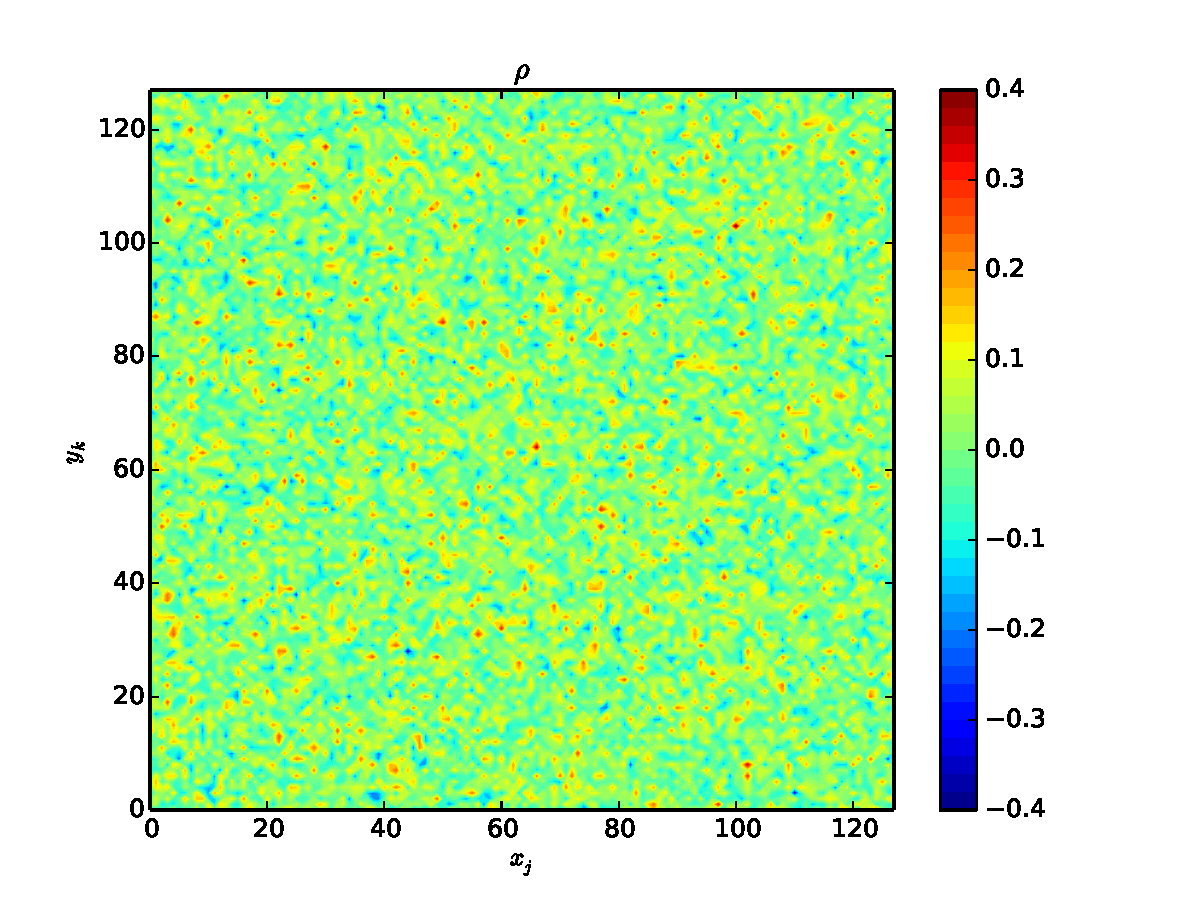
\includegraphics[width = \textwidth]{figures/verification/analytical/random/rho.pdf}
			\end{subfigure}
			\begin{subfigure}[b]{0.6\textwidth}
				\includegraphics[width = \textwidth]{figures/verification/analytical/random/numerical.pdf}
			\end{subfigure}
			\begin{subfigure}[b]{0.6\textwidth}
				\includegraphics[width = \textwidth]{figures/verification/analytical/random/residual.pdf}
			\end{subfigure}
			\caption{As earlier this is a \(x,y\)-plane cut along \(x_k=32\), of the grid. The plots show the charge distribution,
			numerical solution and the solution, from top to bottom. It is visible that the potential shows more structure than
			the \(\rho\), since the integration smooths the original problem.}
			\label{fig:random}
		\end{figure}

	\subsection{Additional Tests}
		In addition to the tests on shown in this section, we also ran the same tests
		obtaining similar results on various sizes and directions. Since we wanted to be sure that the program
		was working independently of the how the domain was divided into subdomains, we also performed
		tests on different subdomain divisions.


	\subsection{ND vs 3D algorithms}
		PINC is built to have two sets of algorithms, one N-dimensional and one 3-dimensional.
		The N-dimensional algorithms is meant to be used in cases where one want to do 1- and 2-dimensional
		simulations as well as a test for the 3-dimensional algorithm. The 3-dimensional algorithm
		is generally slightly faster than the N-dimensional due to some extra capabilities in hardcoding
		certain parts. On a laptop, using two 'Intel(R) Core(TM) i7-4710MQ CPU @ 2.50GHz' processors, we
		ran the multigrid solver on a \(128,128,128\) size problem, with both the \(3\)D and ND algorithms.
 		The ND algorithms used \(80.08\)s to solve it to the given tolerance, while the \(3\)D algorithms
 		used \(78.75\)s achieving only a slight speedup. This is likely due to most of the
		computational time being spent on the interprocessor communication.
